\documentclass{article}
\usepackage{graphicx}
\usepackage{amsmath}
\usepackage{geometry}
\geometry{a4paper, margin=1in, left=1.5in, right=1.5in, top=1in, bottom=1in}
\usepackage{float}
\usepackage{subcaption}
\usepackage{booktabs}
\usepackage{xcolor}
\usepackage{setspace}
\onehalfspacing

% Custom colors
\definecolor{accent}{RGB}{59,90,140}
\definecolor{highlight}{RGB}{200,50,50}

\title{PA3: Comparative Analysis of DCGAN and CycleGAN Performance}
\author{Chen Yuanzhong}
\date{\today}

\begin{document}

\maketitle

\begin{abstract}
This report presents a comparative analysis of Deep Convolutional Generative Adversarial Networks (DCGAN) and Cycle-Consistent Adversarial Networks (CycleGAN) for image generation tasks. Through systematic experimentation, we evaluate model performance via training dynamics and qualitative assessment of generated samples. Key findings include the superior performance of CycleGAN architecture and the observation that optimal results are typically achieved well before the nominal training duration.
\end{abstract}

\section{Introduction}
This investigation examines the relative performance of two prominent generative adversarial network architectures: DCGAN and CycleGAN. The study focuses on:
\begin{itemize}
\item Training dynamics and loss convergence patterns
\item Qualitative assessment of generated samples
\item Comparative analysis of architectural effectiveness
\item Optimization strategies and their impact
\end{itemize}

\section{DCGAN Experiments}
The DCGAN model was trained for 1000 epochs on the emoji dataset, with evaluation metrics recorded throughout the training process.

\subsection{Training Dynamics}
Figure \ref{fig:Training loss in 100 epochs} presents the training loss trajectories for both generator and discriminator components. Several key observations emerge:

\begin{figure}[H]
    \centering
    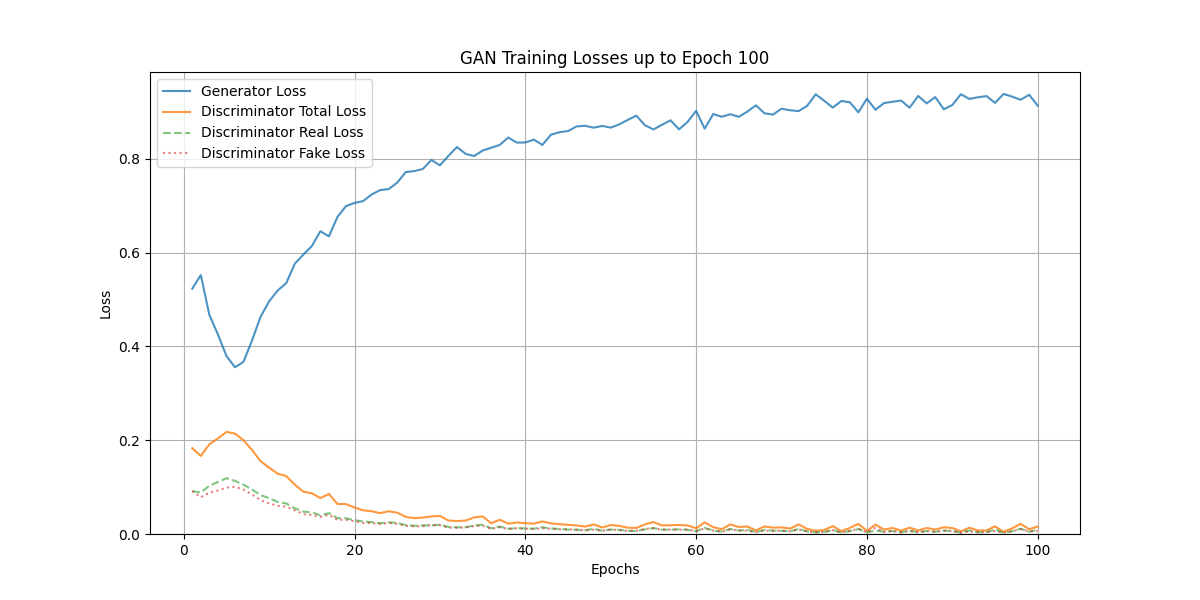
\includegraphics[width=1\linewidth]{loss_plot_epoch_0100.png}
    \caption{Training loss in 100 epochs}
    \label{fig:Training loss in 100 epochs}
\end{figure}

\subsection{Initial Training Phase Analysis}
To better illustrate the training process in GAN, we also present the loss figure for the first 10,400 iterations here. This initial phase often reveals critical dynamics such as early convergence patterns or initial instability.

\begin{figure}[H]
    \centering
    % --- Replace 'loss_plot_first_10400_iterations.png' with your actual image file name ---
    \includegraphics[width=1\linewidth]{placeholder_loss_10400_iterations.png}
    \caption{Training loss during the first 10,400 iterations}
    \label{fig:Training loss first 10400 iterations}
\end{figure}

\subsection{Generated Samples}
Five representative samples generated by the DCGAN model:

\begin{figure}[H]
\centering
\begin{subfigure}{0.32\textwidth}
    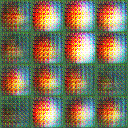
\includegraphics[width=\linewidth]{sample-000200.png}
    \caption{Sample 1}
    \label{fig:dcgan_sample 200 iterations}
\end{subfigure}
\hfill
\begin{subfigure}{0.32\textwidth}
    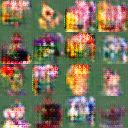
\includegraphics[width=\linewidth]{sample-001000.png}
    \caption{Sample 2}
    \label{fig:dcgan_sample 1000 iterations}
\end{subfigure}
\hfill
\begin{subfigure}{0.32\textwidth}
    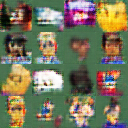
\includegraphics[width=\linewidth]{sample-004000.png}
    \caption{Sample 3}
    \label{fig:dcgan_sample 4000 iterations}
\end{subfigure}
\\
\begin{subfigure}{0.32\textwidth}
    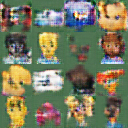
\includegraphics[width=\linewidth]{sample-008000.png}
    \caption{Sample 4}
    \label{fig:dcgan_sample 8000 iterations}
\end{subfigure}
\hfill
\begin{subfigure}{0.32\textwidth}
    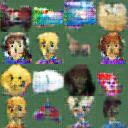
\includegraphics[width=\linewidth]{sample-012600.png}
    \caption{Sample 5}
    \label{fig:dcgan_sample 12600 iterations}
\end{subfigure}
\caption{Five representative samples generated by DCGAN demonstrating the model's output characteristics}
\label{fig:dcgan_samples}
\end{figure}

\section{CycleGAN Experiments}
The CycleGAN model was trained for 100,000 iterations on the Apple-Windows dataset for unpaired image-to-image translation.

\subsection{Loss Component Analysis}
Figure \ref{fig:cyclegan_losses} presents the comprehensive loss trajectories:

\begin{figure}[H]
\centering
\begin{subfigure}{0.8\textwidth}
    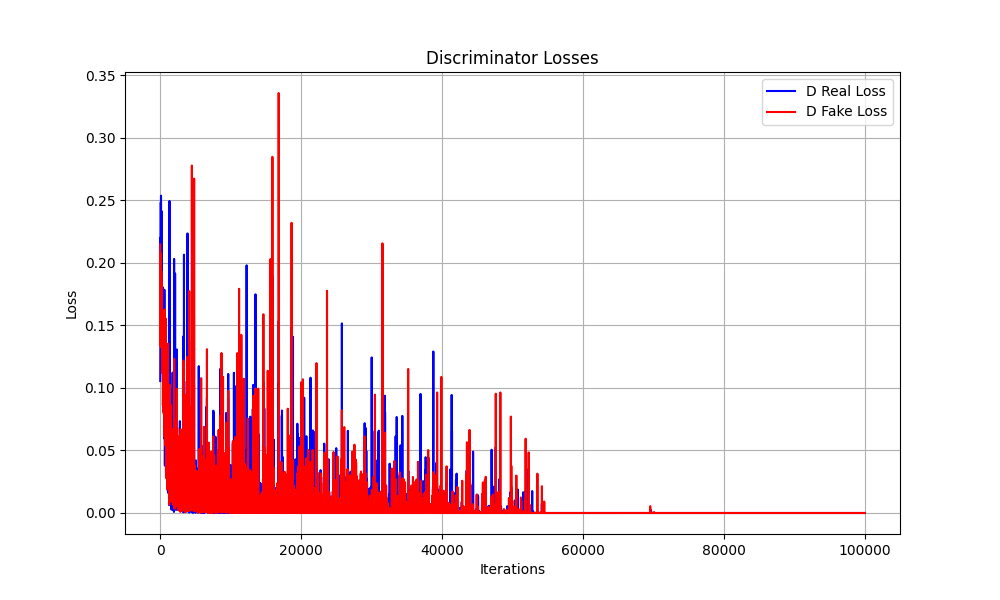
\includegraphics[width=\linewidth]{d_losses_100000.png}
    \caption{Discriminator losses (D\_A and D\_B)}
    \label{fig:cyclegan_d_loss}
\end{subfigure}
\\
\begin{subfigure}{0.8\textwidth}
    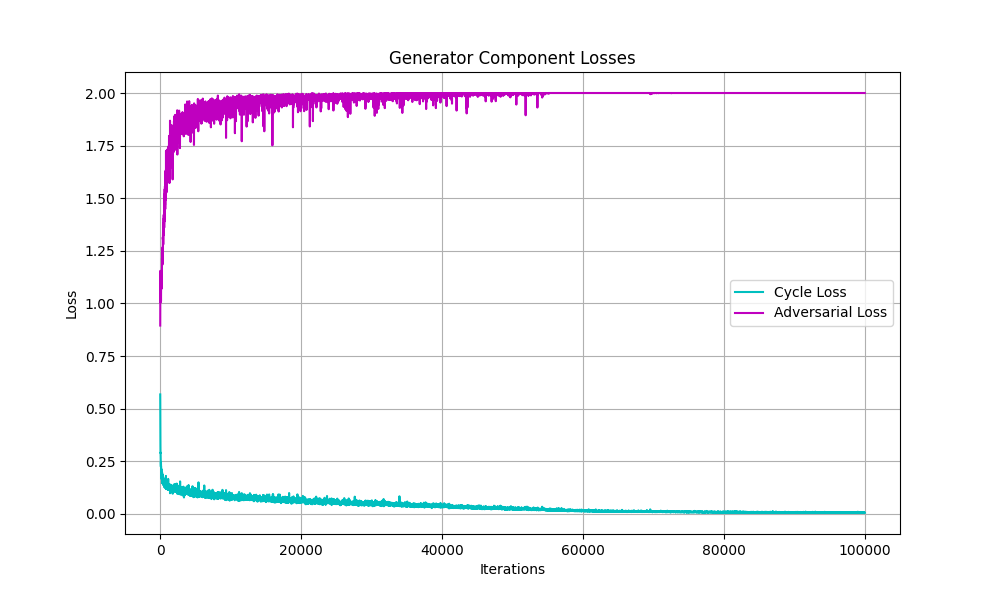
\includegraphics[width=\linewidth]{g_component_losses_100000.png}
    \caption{Generator loss components}
    \label{fig:cyclegan_g_components}
\end{subfigure}
\\
\begin{subfigure}{0.8\textwidth}
    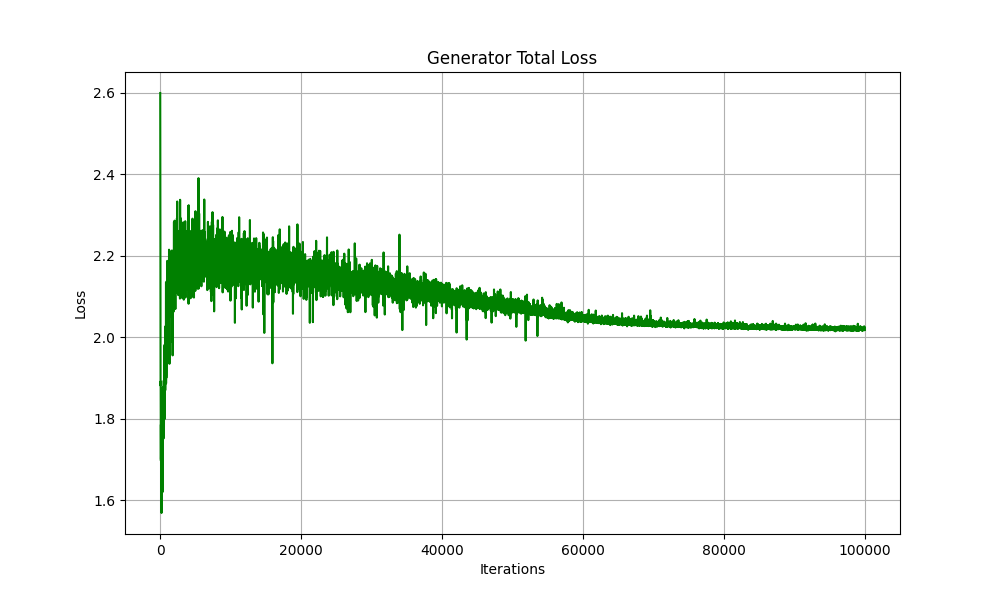
\includegraphics[width=\linewidth]{g_total_loss_100000.png}
    \caption{Total generator loss}
    \label{fig:cyclegan_g_total}
\end{subfigure}
\caption{CycleGAN loss trajectories showing (a) discriminator losses, (b) generator component losses, and (c) total generator loss. The stabilization of metrics after 10,000 iterations indicates convergence.}
\label{fig:cyclegan_losses}
\end{figure}

\subsection{Translation Sample Pairs}
Five representative translation pairs demonstrating the model's bidirectional transformation capability:

\begin{figure}[H]
\centering
\begin{subfigure}{0.45\textwidth}
    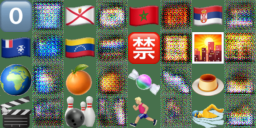
\includegraphics[width=\linewidth]{sample-000100-X-Y.png}
    \caption{Pair 1: X→Y}
    \label{fig:cyclegan_pair1_XY}
\end{subfigure}
\hfill
\begin{subfigure}{0.45\textwidth}
    
\includegraphics[width=\linewidth]{sample-000100-Y-X.png}
    \caption{Pair 1: Y→X}
    \label{fig:cyclegan_pair1_YX}
\end{subfigure}
\caption{CycleGAN translation pair 1 showing bidirectional transformation between domains}
\label{fig:cyclegan_pair1}
\end{figure}

\begin{figure}[H]
\centering
\begin{subfigure}{0.45\textwidth}
    
\includegraphics[width=\linewidth]{sample-001000-X-Y.png}
    \caption{Pair 2: X→Y}
    \label{fig:cyclegan_pair2_XY}
\end{subfigure}
\hfill
\begin{subfigure}{0.45\textwidth}
    
\includegraphics[width=\linewidth]{sample-001000-Y-X.png}
    \caption{Pair 2: Y→X}
    \label{fig:cyclegan_pair2_YX}
\end{subfigure}
\caption{CycleGAN translation pair 2 showing bidirectional transformation between domains}
\label{fig:cyclegan_pair2}
\end{figure}

\begin{figure}[H]
\centering
\begin{subfigure}{0.45\textwidth}
    
\includegraphics[width=\linewidth]{sample-005000-X-Y.png}
    \caption{Pair 3: X→Y}
    \label{fig:cyclegan_pair3_XY}
\end{subfigure}
\hfill
\begin{subfigure}{0.45\textwidth}
    
\includegraphics[width=\linewidth]{sample-005000-Y-X.png}
    \caption{Pair 3: Y→X}
    \label{fig:cyclegan_pair3_YX}
\end{subfigure}
\caption{CycleGAN translation pair 3 showing bidirectional transformation between domains}
\label{fig:cyclegan_pair3}
\end{figure}

\begin{figure}[H]
\centering
\begin{subfigure}{0.45\textwidth}
    
\includegraphics[width=\linewidth]{sample-010000-X-Y.png}
    \caption{Pair 4: X→Y}
    \label{fig:cyclegan_pair4_XY}
\end{subfigure}
\hfill
\begin{subfigure}{0.45\textwidth}
    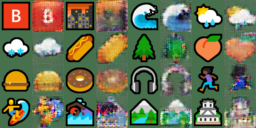
\includegraphics[width=\linewidth]{sample-010000-Y-X.png}
    \caption{Pair 4: Y→X}
    \label{fig:cyclegan_pair4_YX}
\end{subfigure}
\caption{CycleGAN translation pair 4 showing bidirectional transformation between domains}
\label{fig:cyclegan_pair4}
\end{figure}

\section{Conclusion}
Our experimental analysis yields several significant findings:

\begin{itemize}
\item \textbf{Architectural Superiority}: CycleGAN demonstrates consistently better performance than DCGAN, suggesting fundamental advantages in its architecture for image translation tasks.

\item \textbf{Training Efficiency}: Both models achieve optimal performance well before their nominal training durations (DCGAN within 200 epochs, CycleGAN within 10,000 iterations), indicating potential for more efficient training protocols.

\item \textbf{Loss Weighting}: The introduction of weighted loss combinations in CycleGAN (particularly between cycle consistency and adversarial losses) proves effective for performance enhancement.
\end{itemize}

These results suggest that future work should focus on architectural innovations rather than extended training durations, and that careful loss function engineering can yield significant improvements in GAN performance.

\end{document}